\documentclass[11pt,a4paper]{article}

% Packages
\usepackage[utf8]{inputenc}
\usepackage[T1]{fontenc}
\usepackage{amsmath,amssymb}
\usepackage{tikz}
\usepackage{xcolor}
\usepackage{geometry}
\usepackage{float}
\usepackage{caption}
\usepackage{subcaption}
\usepackage{tcolorbox}
\usepackage{enumitem}
\usepackage{listings}
\usepackage{algorithm}
\usepackage{algorithmic}

% TikZ libraries
\usetikzlibrary{arrows.meta, positioning, shapes, calc, decorations.pathreplacing, backgrounds, fit}

% Page geometry
\geometry{margin=2.5cm}

% Custom colors
\definecolor{nodeblue}{RGB}{66, 133, 244}
\definecolor{nodeorange}{RGB}{255, 152, 0}
\definecolor{nodegreen}{RGB}{76, 175, 80}
\definecolor{nodepurple}{RGB}{156, 39, 176}
\definecolor{edgegray}{RGB}{100, 100, 100}
\definecolor{boxblue}{RGB}{227, 242, 253}
\definecolor{boxgreen}{RGB}{232, 245, 233}
\definecolor{boxorange}{RGB}{255, 243, 224}
\definecolor{boxpurple}{RGB}{243, 229, 245}
\definecolor{codebg}{RGB}{245, 245, 245}

% Custom box style
\tcbset{
    parambox/.style={
        colback=#1,
        colframe=#1!50!black,
        boxrule=1pt,
        arc=4mm,
        left=5mm,
        right=5mm,
        top=3mm,
        bottom=3mm
    },
    implbox/.style={
        colback=codebg,
        colframe=edgegray,
        boxrule=0.5pt,
        arc=2mm,
        left=3mm,
        right=3mm,
        top=2mm,
        bottom=2mm,
        fonttitle=\bfseries,
        title=#1
    }
}

% Code listing style
\lstset{
    basicstyle=\ttfamily\small,
    backgroundcolor=\color{codebg},
    breaklines=true,
    frame=single,
    language=Python
}

\title{\textbf{Network Generation Parameters in ASNU}\\[2mm]\large Implementation Documentation}
\author{ASNU Network Analysis}
\date{}

\begin{document}

\maketitle

\section*{Introduction}
This document explains four key parameters used in ASNU's network generation algorithm. Each parameter controls a specific aspect of network topology during edge creation, implemented in the \texttt{establish\_links()} function in \texttt{grn.py}.

%% ============================================
%% PREFERENTIAL ATTACHMENT
%% ============================================
\section{Preferential Attachment (PA)}

\begin{tcolorbox}[parambox=boxblue]
\textbf{Parameter:} \texttt{preferential\_attachment} $\in [0, 1]$\\[2mm]
\textbf{Effect:} Controls whether popular nodes (those already receiving edges) become even more likely to receive additional edges. Higher values create hub-dominated networks.
\end{tcolorbox}

\subsection*{ASNU Implementation}

The implementation uses a \textbf{popularity pool} mechanism. When a node receives an edge, it may be added back to the selection pool, making it more likely to be chosen again.

\begin{tcolorbox}[implbox={Core Logic (grn.py:126-135)}]
\begin{lstlisting}
# After creating edge s -> d_from_db:
if random.uniform(0,1) > fraction and fraction != 1:
    if pa_scope == "global":
        # Add to all community pools
        for comm_id in range(G.number_of_communities):
            G.popularity_pool[(comm_id, dst_id)].append(d_from_db)
    else:
        # Add only to current community's pool
        G.popularity_pool[pool_key].append(d_from_db)
\end{lstlisting}
\end{tcolorbox}

\textbf{Note:} Internally, \texttt{fraction = 1 - preferential\_attachment}. When PA is high (e.g., 0.8), fraction is low (0.2), so the condition \texttt{random > fraction} is often true, causing nodes to be added to the pool frequently.

\subsection*{Visual Explanation}

\begin{figure}[H]
\centering
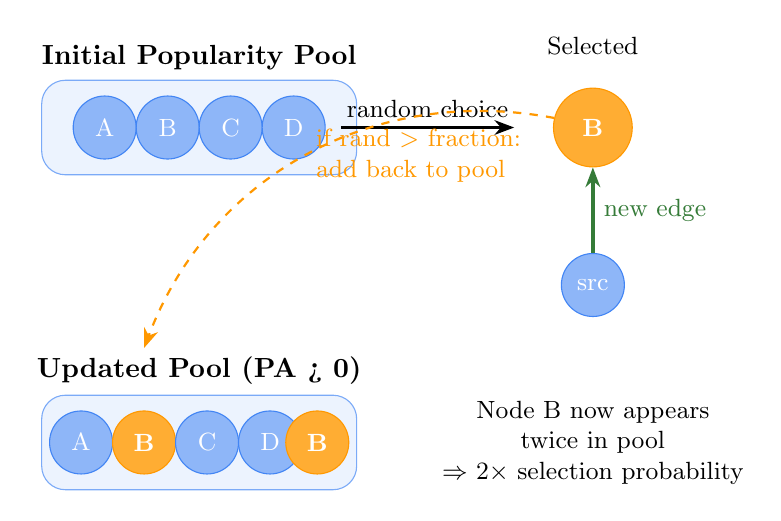
\begin{tikzpicture}[
    node distance=1.2cm,
    pool/.style={rectangle, draw=nodeblue!70, fill=nodeblue!10, minimum width=4cm, minimum height=1.2cm, rounded corners=3mm},
    node/.style={circle, draw=nodeblue, fill=nodeblue!60, minimum size=8mm, font=\small, text=white},
    selectednode/.style={circle, draw=nodeorange, fill=nodeorange!80, minimum size=10mm, font=\small\bfseries, text=white},
    arrow/.style={-{Stealth[length=2.5mm]}, thick},
    dashedarrow/.style={-{Stealth[length=2.5mm]}, thick, dashed, nodeorange}
]

% Initial pool
\node[pool, label=above:{\textbf{Initial Popularity Pool}}] (pool1) at (0,3) {};
\node[node] at (-1.2, 3) {A};
\node[node] at (-0.4, 3) {B};
\node[node] at (0.4, 3) {C};
\node[node] at (1.2, 3) {D};

% Selection
\node[selectednode] (selected) at (5, 3) {B};
\node[above=0.3cm of selected, font=\small] {Selected};

\draw[arrow] (1.8, 3) -- (4, 3) node[midway, above, font=\small] {random choice};

% Edge creation
\node[node] (src) at (5, 1) {src};
\draw[arrow, nodegreen!70!black, very thick] (src) -- (selected) node[midway, right, font=\small] {new edge};

% Updated pool (PA enabled)
\node[pool, label=above:{\textbf{Updated Pool (PA > 0)}}] (pool2) at (0,-1) {};
\node[node] at (-1.5, -1) {A};
\node[selectednode, minimum size=8mm] at (-0.7, -1) {B};
\node[node] at (0.1, -1) {C};
\node[node] at (0.9, -1) {D};
\node[selectednode, minimum size=8mm] at (1.5, -1) {B};

\draw[dashedarrow] (selected) to[bend right=40] node[right, font=\small, align=left] {if rand $>$ fraction:\\add back to pool} (-0.7, 0.2);

% Annotation
\node[align=center, font=\small] at (5, -1) {Node B now appears\\twice in pool\\$\Rightarrow$ 2$\times$ selection probability};

\end{tikzpicture}
\caption{Preferential Attachment: Selected nodes are added back to the popularity pool, increasing their future selection probability.}
\end{figure}

\subsection*{Effect on Network Topology}

\begin{figure}[H]
\centering
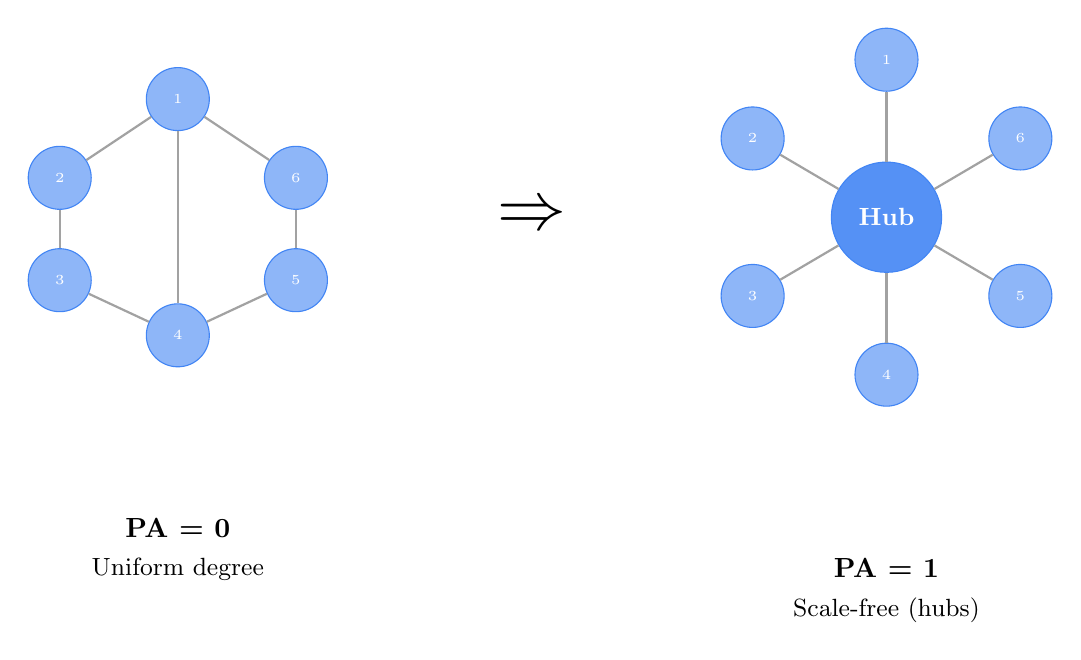
\begin{tikzpicture}[
    node/.style={circle, draw=nodeblue, fill=nodeblue!60, minimum size=8mm, text=white, font=\tiny},
    hub/.style={circle, draw=nodeblue, fill=nodeblue!90, minimum size=14mm, text=white, font=\small\bfseries},
    edge/.style={thick, edgegray!60}
]

% Low PA (left)
\begin{scope}[shift={(-4.5,0)}]
    \node[node] (a1) at (0,1.5) {1};
    \node[node] (a2) at (-1.5,0.5) {2};
    \node[node] (a3) at (-1.5,-0.8) {3};
    \node[node] (a4) at (0,-1.5) {4};
    \node[node] (a5) at (1.5,-0.8) {5};
    \node[node] (a6) at (1.5,0.5) {6};

    \draw[edge] (a1) -- (a2);
    \draw[edge] (a2) -- (a3);
    \draw[edge] (a3) -- (a4);
    \draw[edge] (a4) -- (a5);
    \draw[edge] (a5) -- (a6);
    \draw[edge] (a6) -- (a1);
    \draw[edge] (a1) -- (a4);

    \node[below=1.8cm of a4, font=\bfseries] {PA = 0};
    \node[below=2.3cm of a4, font=\small] {Uniform degree};
\end{scope}

% Arrow
\node[font=\Huge] at (0, 0) {$\Rightarrow$};

% High PA (right)
\begin{scope}[shift={(4.5,0)}]
    \node[hub] (hub) at (0,0) {Hub};
    \node[node] (b1) at (0,2) {1};
    \node[node] (b2) at (-1.7,1) {2};
    \node[node] (b3) at (-1.7,-1) {3};
    \node[node] (b4) at (0,-2) {4};
    \node[node] (b5) at (1.7,-1) {5};
    \node[node] (b6) at (1.7,1) {6};

    \draw[edge] (hub) -- (b1);
    \draw[edge] (hub) -- (b2);
    \draw[edge] (hub) -- (b3);
    \draw[edge] (hub) -- (b4);
    \draw[edge] (hub) -- (b5);
    \draw[edge] (hub) -- (b6);

    \node[below=1.8cm of b4, font=\bfseries] {PA = 1};
    \node[below=2.3cm of b4, font=\small] {Scale-free (hubs)};
\end{scope}

\end{tikzpicture}
\caption{Low PA creates uniform degree distribution; high PA creates hub-dominated scale-free topology.}
\end{figure}

%% ============================================
%% COMMUNITY STRUCTURE
%% ============================================
\newpage
\section{Community Structure}

\begin{tcolorbox}[parambox=boxgreen]
\textbf{Parameter:} \texttt{number\_of\_communities} $\in \mathbb{Z}^+$\\[2mm]
\textbf{Effect:} Partitions nodes into communities. Edges are constrained to form \textbf{only within communities}, creating modular network structure.
\end{tcolorbox}

\subsection*{ASNU Implementation}

Community formation involves three steps:

\textbf{Step 1: Find seed groups} with minimal inter-connections using greedy selection:

\begin{tcolorbox}[implbox={Seed Selection (generate.py:246-268)}]
\begin{lstlisting}
# Find pair of groups with weakest connection
np.fill_diagonal(normalized, np.inf)
min_i, min_j = np.unravel_index(np.argmin(normalized), normalized.shape)
selected_indices.extend([min_i, min_j])

# Iteratively add groups minimally connected to selected ones
while len(selected_indices) < num_communities:
    for candidate in remaining:
        total = normalized[candidate, selected_indices].sum()
        # Keep candidate with minimum total connection
\end{lstlisting}
\end{tcolorbox}

\textbf{Step 2: Assign nodes} to communities probabilistically based on group affinity:

\begin{tcolorbox}[implbox={Node Assignment (generate.py:178-190)}]
\begin{lstlisting}
# Calculate affinity: communities x groups
affinity_matrix = community_matrix @ G.probability_matrix.T
cumulative_matrix = np.cumsum(affinity_matrix, axis=0)

# Fast sampling using searchsorted
community = np.searchsorted(cumulative_matrix[:, group], random_value)

# Update membership
G.communities_to_nodes[(community, group)].append(node)
G.nodes_to_communities[node] = community
\end{lstlisting}
\end{tcolorbox}

\textbf{Step 3: Constrain edges} to form only within communities:

\begin{tcolorbox}[implbox={Edge Constraint (grn.py:76-77, 86-87)}]
\begin{lstlisting}
# Select community for this edge
community_id = community_batch[batch_idx]

# Get source nodes in this community only
src_node_lists[community_id] = G.communities_to_nodes[(community_id, src_id)]
\end{lstlisting}
\end{tcolorbox}

\subsection*{Visual Explanation}

\begin{figure}[H]
\centering
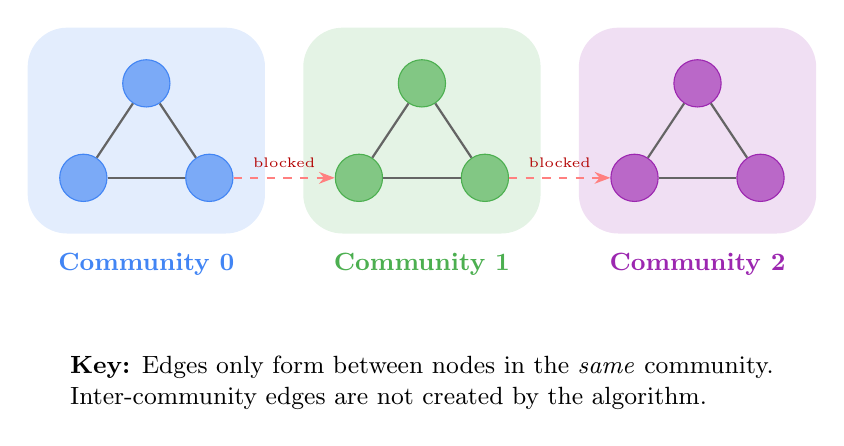
\begin{tikzpicture}[
    node/.style={circle, draw, fill, minimum size=6mm, text=white, font=\tiny},
    nodeA/.style={node, draw=nodeblue, fill=nodeblue!70},
    nodeB/.style={node, draw=nodegreen, fill=nodegreen!70},
    nodeC/.style={node, draw=nodepurple, fill=nodepurple!70},
    intraedge/.style={thick, edgegray},
    blocked/.style={thick, red!50, dashed, -{Stealth[length=2mm]}}
]

% Community A
\begin{scope}[shift={(-3.5,0)}]
    \node[nodeA] (a1) at (0,0.8) {};
    \node[nodeA] (a2) at (-0.8,-0.4) {};
    \node[nodeA] (a3) at (0.8,-0.4) {};

    \draw[intraedge] (a1) -- (a2);
    \draw[intraedge] (a2) -- (a3);
    \draw[intraedge] (a3) -- (a1);

    \begin{scope}[on background layer]
        \node[fit=(a1)(a2)(a3), fill=nodeblue!15, rounded corners=5mm, inner sep=4mm] {};
    \end{scope}
    \node[font=\small\bfseries, nodeblue] at (0, -1.5) {Community 0};
\end{scope}

% Community B
\begin{scope}[shift={(0,0)}]
    \node[nodeB] (b1) at (0,0.8) {};
    \node[nodeB] (b2) at (-0.8,-0.4) {};
    \node[nodeB] (b3) at (0.8,-0.4) {};

    \draw[intraedge] (b1) -- (b2);
    \draw[intraedge] (b2) -- (b3);
    \draw[intraedge] (b3) -- (b1);

    \begin{scope}[on background layer]
        \node[fit=(b1)(b2)(b3), fill=nodegreen!15, rounded corners=5mm, inner sep=4mm] {};
    \end{scope}
    \node[font=\small\bfseries, nodegreen] at (0, -1.5) {Community 1};
\end{scope}

% Community C
\begin{scope}[shift={(3.5,0)}]
    \node[nodeC] (c1) at (0,0.8) {};
    \node[nodeC] (c2) at (-0.8,-0.4) {};
    \node[nodeC] (c3) at (0.8,-0.4) {};

    \draw[intraedge] (c1) -- (c2);
    \draw[intraedge] (c2) -- (c3);
    \draw[intraedge] (c3) -- (c1);

    \begin{scope}[on background layer]
        \node[fit=(c1)(c2)(c3), fill=nodepurple!15, rounded corners=5mm, inner sep=4mm] {};
    \end{scope}
    \node[font=\small\bfseries, nodepurple] at (0, -1.5) {Community 2};
\end{scope}

% Blocked inter-community edges
\draw[blocked] (a3) -- (b2) node[midway, above, font=\tiny, red!70!black] {blocked};
\draw[blocked] (b3) -- (c2) node[midway, above, font=\tiny, red!70!black] {blocked};

% Legend
\node[align=left, font=\small] at (0, -3) {
    \textbf{Key:} Edges only form between nodes in the \textit{same} community.\\
    Inter-community edges are not created by the algorithm.
};

\end{tikzpicture}
\caption{Community structure: nodes are partitioned and edges form only within community boundaries.}
\end{figure}

\subsection*{Community Assignment Flow}

\begin{figure}[H]
\centering
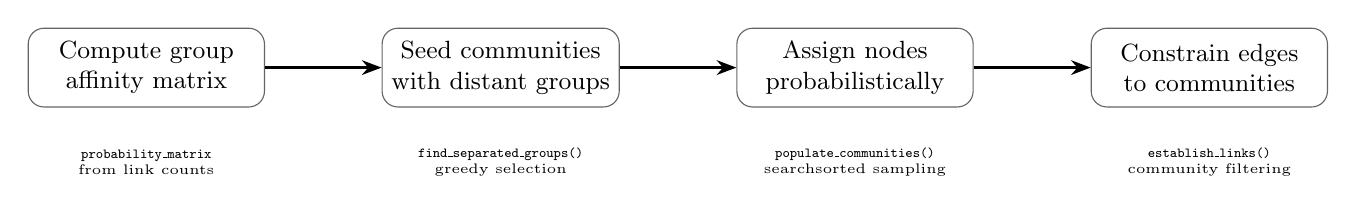
\begin{tikzpicture}[
    box/.style={rectangle, draw=edgegray, fill=white, rounded corners=2mm, minimum height=1cm, align=center, font=\small},
    arrow/.style={-{Stealth[length=2.5mm]}, thick}
]

\node[box, minimum width=3cm] (step1) at (0,0) {Compute group\\affinity matrix};
\node[box, minimum width=3cm] (step2) at (4.5,0) {Seed communities\\with distant groups};
\node[box, minimum width=3cm] (step3) at (9,0) {Assign nodes\\probabilistically};
\node[box, minimum width=3cm] (step4) at (13.5,0) {Constrain edges\\to communities};

\draw[arrow] (step1) -- (step2);
\draw[arrow] (step2) -- (step3);
\draw[arrow] (step3) -- (step4);

% Annotations below
\node[font=\tiny, align=center] at (0, -1.2) {\texttt{probability\_matrix}\\from link counts};
\node[font=\tiny, align=center] at (4.5, -1.2) {\texttt{find\_separated\_groups()}\\greedy selection};
\node[font=\tiny, align=center] at (9, -1.2) {\texttt{populate\_communities()}\\searchsorted sampling};
\node[font=\tiny, align=center] at (13.5, -1.2) {\texttt{establish\_links()}\\community filtering};

\end{tikzpicture}
\caption{Community assignment pipeline in ASNU.}
\end{figure}

%% ============================================
%% RECIPROCITY
%% ============================================
\newpage
\section{Reciprocity}

\begin{tcolorbox}[parambox=boxorange]
\textbf{Parameter:} \texttt{reciprocity} $\in [0, 1]$\\[2mm]
\textbf{Effect:} Probability of creating a reverse edge when an edge is added. When edge $A \rightarrow B$ is created, with probability \texttt{reciprocity}, edge $B \rightarrow A$ is also created.
\end{tcolorbox}

\subsection*{ASNU Implementation}

Reciprocal edges are created immediately after the primary edge, subject to link budget constraints:

\begin{tcolorbox}[implbox={Reciprocity Logic (grn.py:117-123)}]
\begin{lstlisting}
# After adding edge s -> d_from_db:
if random.uniform(0,1) < reciprocity_p:
    # Check if reverse direction has budget remaining
    if G.existing_num_links[(dst_id, src_id)] < G.maximum_num_links[(dst_id, src_id)]:
        if not G.graph.has_edge(d_from_db, s):
            G.graph.add_edge(d_from_db, s)  # Add reverse edge
            G.existing_num_links[(dst_id, src_id)] += 1
\end{lstlisting}
\end{tcolorbox}

The same reciprocity check occurs when transitive edges are created:

\begin{tcolorbox}[implbox={Reciprocity in Transitivity (grn.py:154-160)}]
\begin{lstlisting}
# After adding transitive edge s -> n:
if random.uniform(0,1) < reciprocity_p:
    if not G.graph.has_edge(n, s):
        if G.existing_num_links[(n_id, src_id)] < G.maximum_num_links[(n_id, src_id)]:
            G.graph.add_edge(n, s)  # Add reverse edge
            G.existing_num_links[(n_id, src_id)] += 1
\end{lstlisting}
\end{tcolorbox}

\subsection*{Visual Explanation}

\begin{figure}[H]
\centering
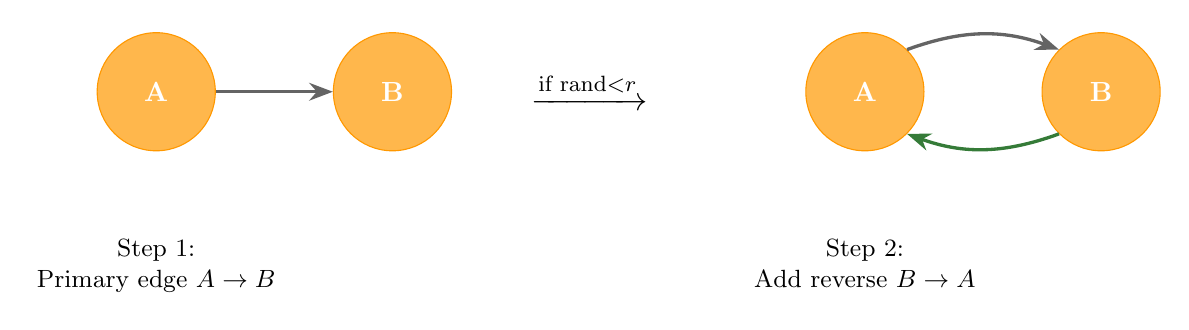
\begin{tikzpicture}[
    node/.style={circle, draw=nodeorange, fill=nodeorange!70, minimum size=15mm, text=white, font=\bfseries},
    arrow/.style={-{Stealth[length=3mm]}, very thick},
    reciparrow/.style={{Stealth[length=3mm]}-{Stealth[length=3mm]}, very thick, nodegreen!80!black}
]

% Step 1: Primary edge
\begin{scope}[shift={(-4,0)}]
    \node[node] (a1) at (0,0) {A};
    \node[node] (b1) at (3,0) {B};

    \draw[arrow, edgegray] (a1) -- (b1);

    \node[below=1cm of a1, anchor=north, font=\small, align=center] {Step 1:\\Primary edge $A \rightarrow B$};
\end{scope}

% Arrow
\node[font=\large] at (1.5, 0) {$\xrightarrow{\text{if rand} < r}$};

% Step 2: With reciprocal edge
\begin{scope}[shift={(5,0)}]
    \node[node] (a2) at (0,0) {A};
    \node[node] (b2) at (3,0) {B};

    \draw[arrow, edgegray] (a2.north east) to[bend left=20] (b2.north west);
    \draw[arrow, nodegreen!70!black] (b2.south west) to[bend left=20] (a2.south east);

    \node[below=1cm of a2, anchor=north, font=\small, align=center] {Step 2:\\Add reverse $B \rightarrow A$};
\end{scope}

\end{tikzpicture}
\caption{Reciprocity: when \texttt{random() < reciprocity\_p}, a reverse edge is created.}
\end{figure}

\subsection*{Reciprocity Check Flowchart}

\begin{figure}[H]
\centering
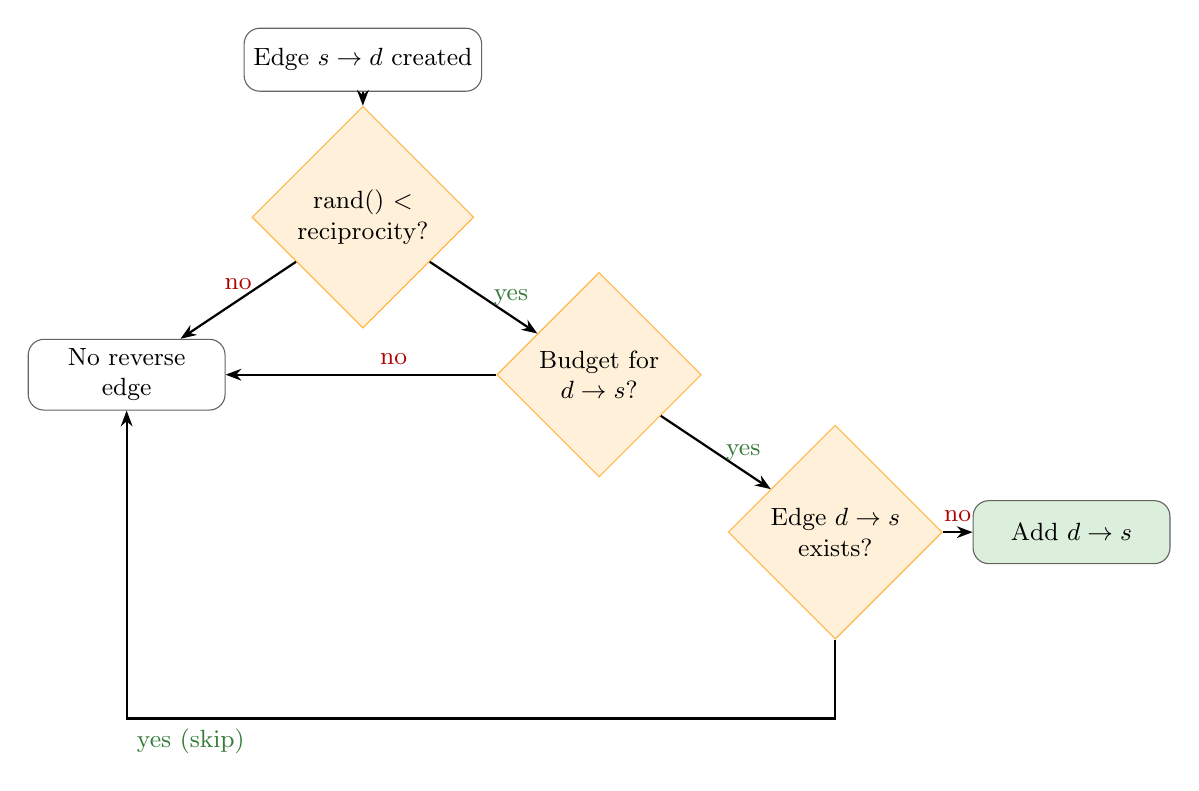
\begin{tikzpicture}[
    decision/.style={diamond, draw=nodeorange!70, fill=nodeorange!15, minimum width=2.5cm, minimum height=1.5cm, align=center, font=\small},
    process/.style={rectangle, draw=edgegray, fill=white, rounded corners=2mm, minimum width=2.5cm, minimum height=0.8cm, align=center, font=\small},
    arrow/.style={-{Stealth[length=2mm]}, thick},
    ymark/.style={font=\small, nodegreen!70!black},
    nmark/.style={font=\small, red!70!black}
]

\node[process] (start) at (0,0) {Edge $s \rightarrow d$ created};

\node[decision] (check1) at (0,-2) {rand() $<$\\reciprocity?};

\node[decision] (check2) at (3,-4) {Budget for\\$d \rightarrow s$?};

\node[decision] (check3) at (6,-6) {Edge $d \rightarrow s$\\exists?};

\node[process, fill=nodegreen!20] (add) at (9,-6) {Add $d \rightarrow s$};

\node[process] (skip) at (-3,-4) {No reverse\\edge};

\draw[arrow] (start) -- (check1);
\draw[arrow] (check1) -- node[ymark, right] {yes} (check2);
\draw[arrow] (check1) -- node[nmark, above] {no} (skip);
\draw[arrow] (check2) -- node[ymark, right] {yes} (check3);
\draw[arrow] (check2.west) -- ++(-1,0) |- node[nmark, above left] {no} (skip);
\draw[arrow] (check3) -- node[nmark, above] {no} (add);
\draw[arrow] (check3.south) -- ++(0,-1) -| node[ymark, below right] {yes (skip)} (skip.south);

\end{tikzpicture}
\caption{Decision flow for reciprocal edge creation.}
\end{figure}

%% ============================================
%% TRANSITIVITY
%% ============================================
\newpage
\section{Transitivity}

\begin{tcolorbox}[parambox=boxpurple]
\textbf{Parameter:} \texttt{transitivity} $\in [0, 1]$\\[2mm]
\textbf{Effect:} Probability of connecting a source node to the \textbf{neighbors} of its destination. When edge $A \rightarrow B$ is created, with probability \texttt{transitivity}, edges $A \rightarrow N$ are created for each neighbor $N$ of $B$.
\end{tcolorbox}

\subsection*{ASNU Implementation}

After each primary edge, the algorithm iterates through the destination's neighbors and potentially creates edges to them:

\begin{tcolorbox}[implbox={Transitivity Logic (grn.py:138-160)}]
\begin{lstlisting}
# After adding edge s -> d_from_db:
if transitivity_p < random.uniform(0,1):
    continue  # Skip transitivity with probability (1 - transitivity_p)

# Create edges to neighbors of destination
for n in G.graph.neighbors(d_from_db):
    if s == n:  # Skip self-loops
        continue
    n_id = G.nodes_to_group[n]

    # Check if this group pair has budget
    if (src_id, n_id) in G.maximum_num_links:
        if G.existing_num_links[(src_id, n_id)] < G.maximum_num_links[(src_id, n_id)]:
            if not G.graph.has_edge(s, n):
                G.graph.add_edge(s, n)  # Transitive edge
                G.existing_num_links[(src_id, n_id)] += 1

                # Reciprocity also applies to transitive edges
                if random.uniform(0,1) < reciprocity_p:
                    # ... add reverse edge n -> s
\end{lstlisting}
\end{tcolorbox}

\subsection*{Visual Explanation}

\begin{figure}[H]
\centering
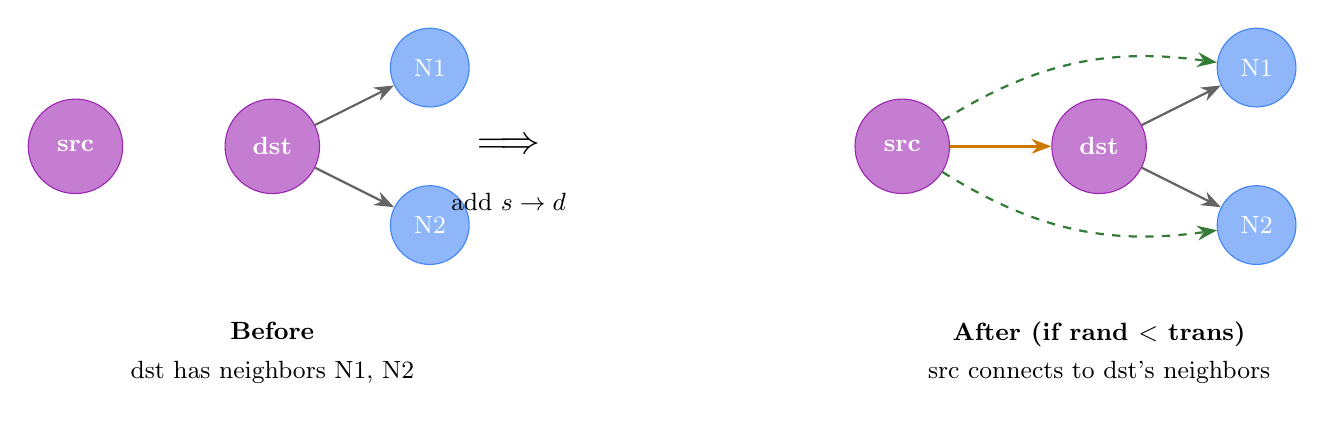
\begin{tikzpicture}[
    node/.style={circle, draw=nodepurple, fill=nodepurple!60, minimum size=12mm, text=white, font=\small\bfseries},
    neighbor/.style={circle, draw=nodeblue, fill=nodeblue!60, minimum size=10mm, text=white, font=\small},
    arrow/.style={-{Stealth[length=2.5mm]}, thick},
    newarrow/.style={-{Stealth[length=2.5mm]}, thick, nodegreen!70!black, dashed}
]

% Step 1: Initial state
\begin{scope}[shift={(-5,0)}]
    \node[node] (s1) at (0,0) {src};
    \node[node] (d1) at (2.5,0) {dst};
    \node[neighbor] (n1a) at (4.5,1) {N1};
    \node[neighbor] (n1b) at (4.5,-1) {N2};

    % Existing edges
    \draw[arrow, edgegray] (d1) -- (n1a);
    \draw[arrow, edgegray] (d1) -- (n1b);

    \node[below=1.5cm of d1, font=\small\bfseries] {Before};
    \node[below=2cm of d1, font=\small] {dst has neighbors N1, N2};
\end{scope}

% Arrow
\node[font=\Large] at (0.5, 0) {$\Longrightarrow$};
\node[font=\small] at (0.5, -0.7) {add $s \rightarrow d$};

% Step 2: After primary edge
\begin{scope}[shift={(5.5,0)}]
    \node[node] (s2) at (0,0) {src};
    \node[node] (d2) at (2.5,0) {dst};
    \node[neighbor] (n2a) at (4.5,1) {N1};
    \node[neighbor] (n2b) at (4.5,-1) {N2};

    % Existing edges
    \draw[arrow, edgegray] (d2) -- (n2a);
    \draw[arrow, edgegray] (d2) -- (n2b);

    % New primary edge
    \draw[arrow, nodeorange!80!black, very thick] (s2) -- (d2);

    % Transitive edges (dashed green)
    \draw[newarrow] (s2) to[bend left=20] (n2a);
    \draw[newarrow] (s2) to[bend right=20] (n2b);

    \node[below=1.5cm of d2, font=\small\bfseries] {After (if rand $<$ trans)};
    \node[below=2cm of d2, font=\small] {src connects to dst's neighbors};
\end{scope}

\end{tikzpicture}
\caption{Transitivity: when creating edge src$\rightarrow$dst, also create edges to dst's existing neighbors.}
\end{figure}

\subsection*{Triangle Formation}

\begin{figure}[H]
\centering
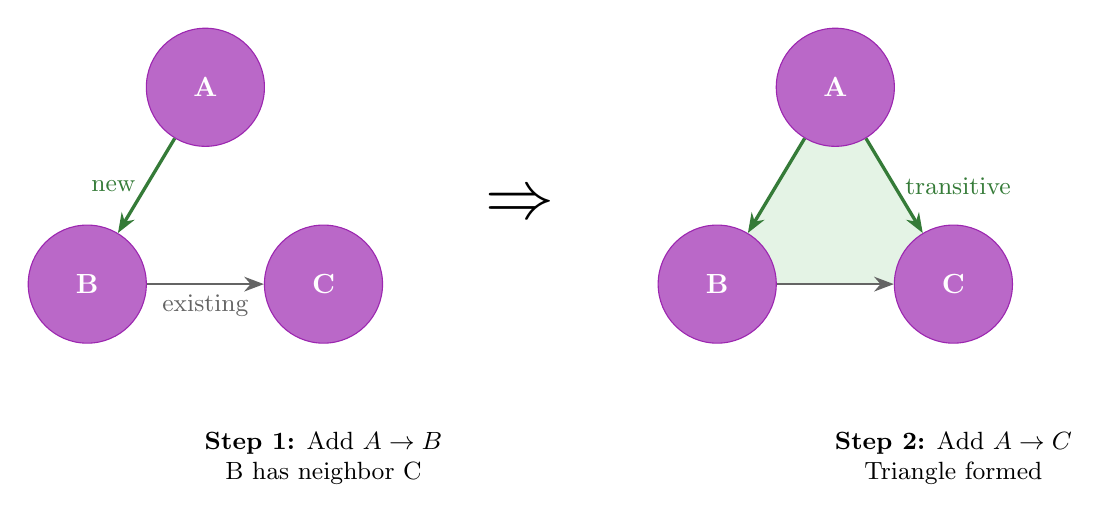
\begin{tikzpicture}[
    node/.style={circle, draw=nodepurple, fill=nodepurple!70, minimum size=15mm, text=white, font=\bfseries},
    arrow/.style={-{Stealth[length=2.5mm]}, thick, edgegray},
    newarrow/.style={-{Stealth[length=2.5mm]}, very thick, nodegreen!70!black}
]

% Open triple
\begin{scope}[shift={(-4,0)}]
    \node[node] (a) at (0,2) {A};
    \node[node] (b) at (-1.5,-0.5) {B};
    \node[node] (c) at (1.5,-0.5) {C};

    % B already connected to C
    \draw[arrow] (b) -- (c) node[midway, below, font=\small] {existing};

    % New edge A -> B
    \draw[newarrow] (a) -- (b) node[midway, left, font=\small] {new};

    \node[below=1cm of c, font=\small, align=center] {\textbf{Step 1:} Add $A \rightarrow B$\\B has neighbor C};
\end{scope}

% Arrow
\node[font=\Huge] at (0,0.5) {$\Rightarrow$};

% Closed triangle
\begin{scope}[shift={(4,0)}]
    \node[node] (a2) at (0,2) {A};
    \node[node] (b2) at (-1.5,-0.5) {B};
    \node[node] (c2) at (1.5,-0.5) {C};

    \draw[arrow] (b2) -- (c2);
    \draw[newarrow] (a2) -- (b2);
    \draw[newarrow] (a2) -- (c2) node[midway, right, font=\small] {transitive};

    % Triangle highlight
    \begin{scope}[on background layer]
        \fill[nodegreen!15] (a2.center) -- (b2.center) -- (c2.center) -- cycle;
    \end{scope}

    \node[below=1cm of c2, font=\small, align=center] {\textbf{Step 2:} Add $A \rightarrow C$\\Triangle formed};
\end{scope}

\end{tikzpicture}
\caption{Transitivity creates triangles by connecting sources to their destinations' neighbors.}
\end{figure}

%% ============================================
%% SUMMARY
%% ============================================
\newpage
\section*{Summary: Parameter Interaction}

\begin{figure}[H]
\centering
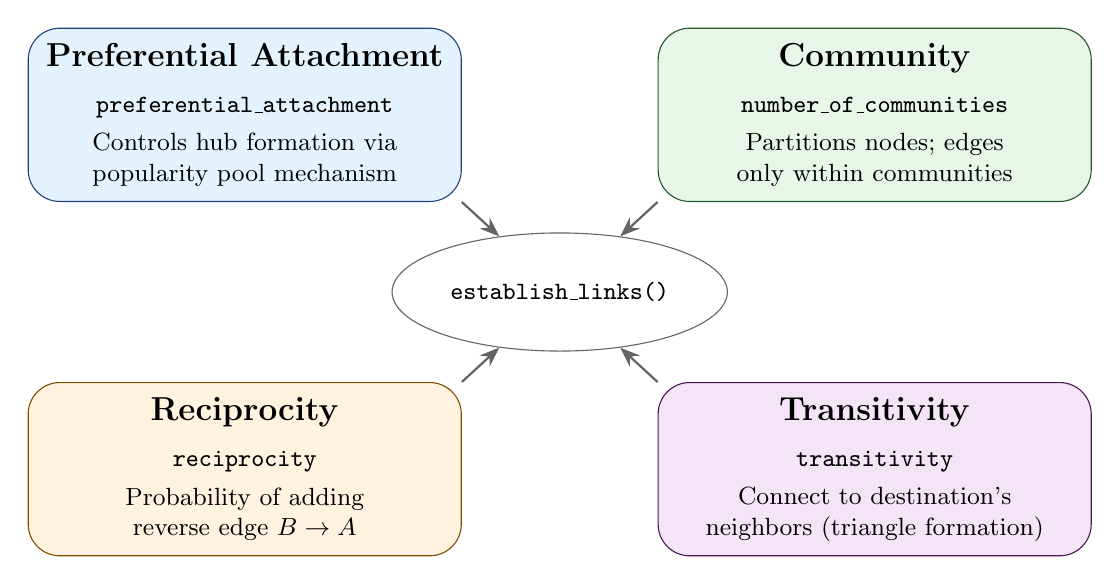
\begin{tikzpicture}[
    box/.style={rectangle, rounded corners=4mm, minimum width=5.5cm, minimum height=2.2cm, align=center, font=\small},
    arrow/.style={-{Stealth[length=2.5mm]}, thick, edgegray}
]

% PA box
\node[box, fill=boxblue, draw=nodeblue!50!black] (pa) at (-4,3.5) {
    \textbf{\large Preferential Attachment}\\[2mm]
    \texttt{preferential\_attachment}\\[1mm]
    Controls hub formation via\\popularity pool mechanism
};

% Community box
\node[box, fill=boxgreen, draw=nodegreen!50!black] (comm) at (4,3.5) {
    \textbf{\large Community}\\[2mm]
    \texttt{number\_of\_communities}\\[1mm]
    Partitions nodes; edges\\only within communities
};

% Reciprocity box
\node[box, fill=boxorange, draw=nodeorange!50!black] (recip) at (-4,-1) {
    \textbf{\large Reciprocity}\\[2mm]
    \texttt{reciprocity}\\[1mm]
    Probability of adding\\reverse edge $B \rightarrow A$
};

% Transitivity box
\node[box, fill=boxpurple, draw=nodepurple!50!black] (trans) at (4,-1) {
    \textbf{\large Transitivity}\\[2mm]
    \texttt{transitivity}\\[1mm]
    Connect to destination's\\neighbors (triangle formation)
};

% Center: establish_links
\node[ellipse, draw=edgegray, fill=white, minimum width=3.5cm, minimum height=1.5cm, font=\small\bfseries] (center) at (0,1.25) {\texttt{establish\_links()}};

% Connecting arrows
\draw[arrow] (pa.south east) -- (center);
\draw[arrow] (comm.south west) -- (center);
\draw[arrow] (recip.north east) -- (center);
\draw[arrow] (trans.north west) -- (center);

\end{tikzpicture}
\caption{All four parameters are applied in \texttt{establish\_links()} during edge creation.}
\end{figure}

\begin{table}[H]
\centering
\renewcommand{\arraystretch}{1.6}
\begin{tabular}{|l|c|c|p{5.5cm}|}
\hline
\textbf{Parameter} & \textbf{Range} & \textbf{Location} & \textbf{Implementation Mechanism} \\
\hline
\texttt{preferential\_attachment} & $[0, 1]$ & grn.py:126 & Node added back to popularity pool with prob. PA \\
\hline
\texttt{number\_of\_communities} & $\mathbb{Z}^+$ & generate.py:280 & Nodes partitioned; edges constrained to communities \\
\hline
\texttt{reciprocity} & $[0, 1]$ & grn.py:117 & Reverse edge created with probability $r$ \\
\hline
\texttt{transitivity} & $[0, 1]$ & grn.py:138 & Edges to dst's neighbors with probability $t$ \\
\hline
\end{tabular}
\caption{Summary of network generation parameters in ASNU.}
\end{table}

\subsection*{Edge Creation Order}

\begin{enumerate}[noitemsep]
    \item \textbf{Select community} from valid communities for the group pair
    \item \textbf{Select source and destination} nodes from community's popularity pool
    \item \textbf{Create primary edge} $s \rightarrow d$
    \item \textbf{Reciprocity check:} if \texttt{rand() < reciprocity}, add $d \rightarrow s$
    \item \textbf{Preferential attachment:} if \texttt{rand() > (1-PA)}, add $d$ back to pool
    \item \textbf{Transitivity check:} if \texttt{rand() < transitivity}, for each neighbor $n$ of $d$:
    \begin{itemize}[noitemsep]
        \item Add edge $s \rightarrow n$ (if budget allows)
        \item Apply reciprocity check for $n \rightarrow s$
    \end{itemize}
\end{enumerate}

\end{document}
